%%%%%%%%%%%%%%%%%%%%%%%%%%%%%%%%%%%%%%%%%%%%%%%%%%%%%%%%%%%%%%%%%%%%%%%%
%%
%% 序論.tex
%% LaTeX-2e 専用
%% 
%% 
%%        設計工学研究室 学位論文テンプレート
%%
%%                      作成日時    2010年 12月 17日
%%
%%%%%%%%%%%%%%%%%%%%%%%%%%%%%%%%%%%%%%%%%%%%%%%%%%%%%%%%%%%%%%%%%%%%%%%%

\chapter{序論}\label{chapter:序論}
第\ref{chapter:序論}章では,本研究の研究背景と先行研究,そして研究の目的を述べる.


\section{背景}
近年,人間に代わって作業を行う移動ロボットの導入が進められている.
これらのロボットの多くはタイヤやホイールを用いての移動を行うが,その他の移動様式として,脚を使用して移動を行う多脚ロボットが存在する.
多脚ロボットは他の移動様式を用いて移動するロボットに比べて,障害物をまたいで超えることが可能な点や,離散的に接地点を選択できる点において優れているといえる.

実際に,林業を行う山間地において多脚ロボットの導入を

このような不整地において,多脚ロボットを使用する場合は適切な歩容計画を行う必要がある.
歩容計画には,カムやリンクを用いて,周期的に脚を動かす固定歩容と,
非周期的に脚を動かす自由歩容がある.

当研究室で行われてきた先行研究では,

\section{本研究の目的}
これまでの研究によって,3次元の不整地において,重心高さを変更しつつ,
自由歩容パターン生成を行うことが可能となった.
しかし低頻度ではあるが,グラフ探索に成功したとしても,
その歩容パターン通りに歩行することができずに動作を停止してしまう問題が生じてしまった.

そこで本論文では,常に脚軌道生成に成功するような歩容パターン生成手法を提案し,
脚軌道生成の失敗による動作停止を防ぐことを目的とする.

\section{本論文の構成}
本論文は,全6章から構成される.

第2章「歩容パターンの再評価手法の提案」では,~を述べる.
第3章「実験装置や開発機械」では,~を述べる.
第4章「実験」では,~を述べる.
第5章「結論」では本論文の結論と今後の課題を述べる.

% \section{other}
% 図の参照はFig. \ref{fig:sample}とする.

% 表の参照はTab. \ref{table:sample}とする.

% 参考文献の参照は\cite{実用的4足歩行機械}とする.



% %図の挿入例
% \begin{figure}[tbp]
%   \begin{center}
%     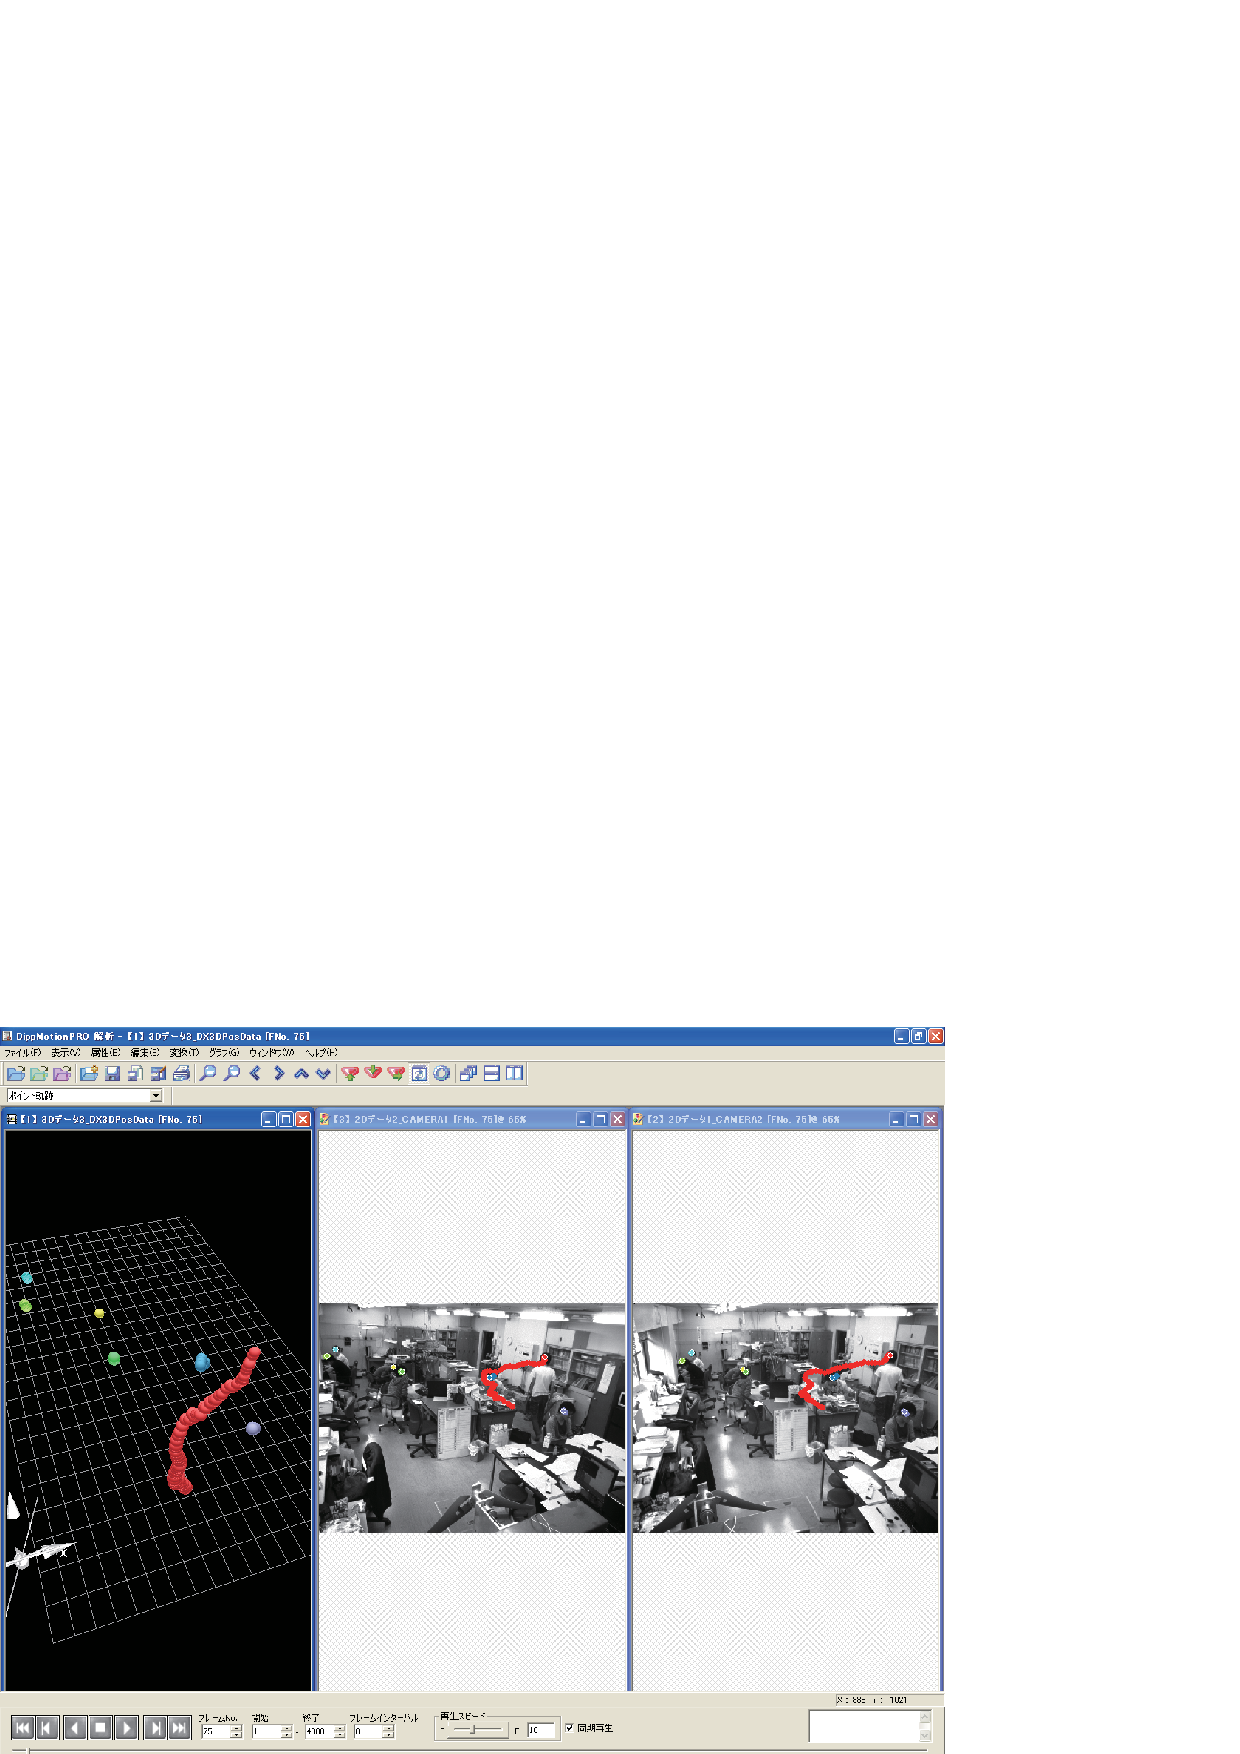
\includegraphics[width=50mm, clip]{figure1/sample.jpg}
%     \caption{Sample figure}
%     \label{fig:sample}
%   \end{center}
% \end{figure}

% %表の挿入例
% \begin{table}[tbp]
%     \caption{Sample table}
%     \label{table:sample}
%     \begin{center}
%         \begin{tabular} {|c|c|c|}
%         \hline
%         Item & Spec. & Quantity  \\
%         \hline\hline
%         A & high & 10 \\
%         \hline
%         B & low & 100 \\
%         \hline
%         \end{tabular}
%     \end{center}
% \end{table}
